\documentclass[12pt,a4paper,oneside]{report}
\usepackage{enumitem}
\usepackage{xcolor}
%\usepackage{sectsty}
\usepackage{longtable}
\usepackage{caption}
\usepackage{subcaption}
\usepackage{float}
\usepackage{graphicx}
\usepackage{tabularray}
\usepackage{array}
\usepackage{setspace}
\usepackage{tocloft}
\usepackage[nottoc]{tocbibind}
\usepackage{amsmath}
\usepackage{amsfonts}
\usepackage{amssymb}
\usepackage{makeidx}
\usepackage{multirow}
\usepackage[left=1in,right=1in,top=1in,bottom=1in]{geometry}
\usepackage[super,square,sort,comma,numbers]{natbib}
\usepackage[version=4]{mhchem}

%\chapternumberfont{\normalsize} 
%\chaptertitlefont{\LARGE}
%\sectionfont{\large}

\setlength{\extrarowheight}{2pt}

\renewcommand{\thefootnote}{\fnsymbol{footnote}}
\renewcommand{\contentsname}{\Large CONTENTS}
\renewcommand{\cftfigfont}{Figure }
\renewcommand{\cfttabfont}{Table }
\renewcommand{\cftdot}{}
\graphicspath{{./images/}}

\setcitestyle{square}
\pagenumbering{roman}
\date{}

\begin{document}
\thispagestyle{empty}
\begin{center}
{\Large  \MakeUppercase{\bf Automation of DevOps Processes}\\} 
\vspace{0.8cm}
{\Large  \MakeUppercase{\bf Long-Term Internship Report}\\}
\doublespacing
\vspace*{2.5cm}
{\normalsize \it A report submitted in partial fulfillment of the requirements for award of the Degree of\\
}
{\bf BACHELOR OF TECHNOLOGY }\\
{\bf in }\\
{\bf COMPUTER SCIENCE ENGINEERING }\\
{\bf by }\\
\vspace*{1cm}
{\bf\textcolor{blue} {BALINENI SREEDHAR NAIDU }}\\
{\bf \textcolor{blue}{ID: N180058}} \\
{\bf Under supervision of }\\
{\bf Mr. Venkata Narasimha Kowru, SaYukth}\\
{\bf Technologies Pvt Ltd,Hyderabad} \\
{\bf 11 Sep, 2023 to 15 Mar, 2024} \\ 
{\bf Major Project Guide: Mr. Kalapala Sravan Kumar } \\

\vspace*{0.8cm}
\begin{figure}[hbt]
\centering
\vspace*{0.6cm}
\centerline{
\includegraphics[scale=0.29]{images/rgukt.png}}
\end{figure}
\vspace*{0.3cm}
{\small \bf DEPARTMENT OF COMPUTER SCIENCE ENGINEERING}\\
{\small \bf RAJIV GANDHI UNIVERSITY OF KNOWLEDGE TECHNOLOGIES}\\
{\small \bf NUZVID, INDIA\\ }
\end{center}
\newpage
\thispagestyle{empty}
\vspace*{1cm}
\begin{center}{\large \bf DECLARATION}\end{center}
\vspace{1cm}
\setstretch{1.5}
\hspace{1cm}I, \textbf{Balineni Sreedhar Naidu}  hereby declare that the long-term project report is submitted for partial fulfilment of the requirements for the award of the degree of Bachelor of Technology in Computer Science Engineering of the Rajiv Gandhi University of Knowledge Technologies, Nuzvid is a bonafide work done by me under the supervision of\\ \textbf{Mr. Venkata Narasimha Kowru}, Team Leader at SaYukth Technologies Pvt Ltd,Hyderabad, and under the guidance of \textbf{Mr. Kalapala Sravan Kumar }. This submission represents my ideas in my own words and where ideas or words of others have been included, I have adequately and accurately cited and referenced the original sources. I also declare that I have adhered to the ethics of academic honesty and integrity and have not misrepresented or fabricated any data or idea or fact or source in my submission. I understand that any violation of the above will be a cause for disciplinary action by the institute and/or the University and can also evoke penal action from the sources which have thus not been properly cited or from whom proper permission has not been obtained. This report has not been previously formed as the basis for the award of any degree, diploma, or similar title of any other University.
\\
\vspace{1cm} \\
...............................\\
Internal Examiner :\\
Date : \\
\vspace{1cm} \\
\textbf{Balineni Sreedhar Naidu (N180058)}  



\newpage
\pagenumbering{roman}
\thispagestyle{empty}

\setstretch{1.25}
\begin{center}
{\large \bf DEPARTMENT OF COMPUTER SCIENCE ENGINEERING}\\
{\large \bf RAJIV GANDHI UNIVERSITY OF KNOWLEDGE TECHNOLOGIES,}
{\large \bf NUZVID, INDIA}\vspace{0.1cm}\end{center}

\begin{figure}[hbt]
\centering
\centerline{
\includegraphics[scale=0.25]{images/rgukt.png}}
\end{figure}

\begin{center} 
\addcontentsline{toc}{chapter}{Certificate}
{\Large  \textbf{CERTIFICATE}}\end{center}
\begin{spacing}{1.5}
This is to certify that the report entitled \textbf{"Automation of DevOps Processes"} submitted by \textbf{Balineni Sreedhar Naidu (N180058)} to the Rajiv Gandhi University of Knowledge Technologies, Nuzvid in partial fulfilment of the requirements for the award of the Degree of Bachelor of Technology in Computer Science Engineering is a bonafide record of the project work carried out by him under our guidance and supervision. This report in any form has not been submitted to any other University or Institute for any purpose.\end{spacing}
\vspace{2cm}
\noindent
\begin{tabular}[t]{@{}l}
\textbf{Mr. Kumar Anurupam }\\ Internal Supervisor\\Professor\\Dept. of Computer Science Engineering \\RGUKT NUZVID6
\end{tabular}
\hfill
\begin{tabular}[t]{@{}r}
\textbf{Mr. R. Siva Narayana}\\External Supervisor\\Asst.Professor\\Dept. of Computer Science Engineering\\RGUKT NUZVID
\end{tabular}



\vspace{2cm}
\noindent
\begin{tabular}[t]{@{}l}
\textbf{Mr. B. Mahalakshmi Rao}\\External Supervisor\\Asst.Professor\\Dept. of Computer Science Engineering\\RGUKT NUZVID
\end{tabular}
\hfill
\begin{tabular}[t]{@{}r}
\textbf{Dr. D.V. Nagarjuna Devi}\\Head of the Department\\Dept. of Computer Science Engineering \\RGUKT NUZVID
\end{tabular}

% \vspace{2cm}
% \noindent
% \begin{tabular}[t]{@{}l} 
% \textbf{Mr. S. Chiranjeevi}\\Head of the Department\\Dept. of Computer Science Engineering \\RGUKT NUZVID
% \end{tabular}
% \hfill
% \begin{tabular}[t]{@{}r} 
% \end{tabular}




\newpage

\thispagestyle{empty}
\vspace*{3cm}
\addcontentsline{toc}{chapter}{Acknowledgement}
\begin{center}  {\large \bf ACKNOWLEDGEMENT}\end{center}
\vspace{1cm}
\setstretch{1.5}
\hspace{1cm}We express our sincere gratitude towards our Manager \textbf{Mr.Venkata Narasimha Kowru}, SaYukth Technologies Pvt Ltd, and our guide \textbf{Mr.Kalapala Sravan Kumar},
Computer Science Engineering, Rajiv Gandhi University of Knowledge Technologies for his valuable guidance, suggestions, and supervision throughout the work. Without his patronage and guidance, the project would not have taken shape. We would also like to express our regards for his kind approval of the project, time-to-time counseling, and advice. We owe our sincere thanks to the Dept.of Computer Science Engineering, Rajiv Gandhi University of Knowledge Technologies. 
\newpage
\vspace*{2cm}
\addcontentsline{toc}{chapter}{Abstract}
\begin{center}  {\Large \bf ABSTRACT}\end{center}
\vspace{1cm}
\noindent 
\hspace{1cm}
Introducing Intelligent  Search Assist a personalized cognitive search assistant designed to provide instantaneous user support and information retrieval. By leveraging the Manage Content stage, data retrieval is seamlessly executed from diverse sources like file uploads, website crawls, and FAQs, Youtube Video, Google drive and Images ensuring streamlined organization for efficient search operations. The project's primary objective is to redefine user interaction by delivering personalized and contextually relevant information in real-time, utilizing state-of-the-art Large Language Models (LLMs). Moreover, Intelligent search Assist is equipped to directly deliver answers to user queries from their own knowledge base, thereby enhancing the efficiency and effectiveness of user support processes..
\setstretch{1.3}


\newpage
\thispagestyle{empty}

\newpage
\tableofcontents 	
\cleardoublepage 

% \listoftables 	\cleardoublepage 
\listoffigures 	\cleardoublepage

\newpage
\begin{center}  {\Large \bf ABBREVIATIONS}\end{center}
\vspace{1cm}\doublespacing
\begin{tabular}{l l}

AI & Artificial Intelligence \\
RAG & Retrieval augmented generation  \\
LLM & Large Language Model \\


\end{tabular} 

\newpage
\pagenumbering{arabic}
\chapter{Introduction}

\hspace{1cm}Introducing our proposed method for Intelligent Search Assistant, a revolutionary approach to enhancing user interaction and information retrieval. At its core, our method leverages advanced techniques such as Retrieval-Augmented Generation (RAG) with Large Language Models (LLMs). By combining retrieval-based techniques with generative capabilities, we aim to provide users with personalized answers directly from their own knowledge base. This approach ensures that users have access to contextually relevant information tailored to their specific queries and needs.\\
\\
\hspace{1cm}    To efficiently manage and retrieve information, we employ the LangChain framework in conjunction with vector databases. LangChain, a versatile Python library, plays a crucial role in breaking down text from various document formats, such as PDFs, Word documents, and plain text files. Through LangChain's text segmentation capabilities and the utilization of Sentence Transformer, we transform document text into compact yet information-rich embeddings. These embeddings serve as the foundation for efficient storage and retrieval of relevant information during user interactions.\\
\\
\hspace{1cm}Furthermore, our method integrates seamlessly with databases and platforms like Google Drive, expanding the scope of accessible information sources. This integration enables users to retrieve information not only from traditional documents but also from websites, YouTube videos, and other multimedia sources. By providing users with a comprehensive range of information sources, we empower them to find answers to their queries more effectively and efficiently. \\
\\
\hspace{1cm}In practice, when users submit queries or prompts, our system utilizes the combined power of RAG techniques with LLMs to generate personalized responses. This ensures that users receive accurate and contextually relevant information in real-time. Additionally, the system maintains a record of previous interactions and chat history, fostering continuity and coherence in the user's dialogue with the Intelligent Search Assistant. Overall, our method aims to revolutionize information retrieval, enhancing user autonomy and efficiency in accessing knowledge from diverse sources..\\



 
\newpage
\chapter{Background and Related Work}
\hspace{1cm}
Traditional chatbot systems have primarily relied on rule-based approaches for generating responses, where fixed rules dictate the bot's behavior and the corresponding answers it provides. However, such rule-based assistants are inherently limited in their flexibility and adaptability. They struggle to handle complex queries and often provide generic or predefined responses, leading to a lack of context and personalized interaction.


In contrast, some chatbots utilize separate Natural Language Processing (NLP) engines for understanding user queries and generating responses. While these systems leverage advanced NLP models, they often suffer from integration challenges. External NLP engines may not seamlessly integrate with the chatbot interface, resulting in disjointed user experiences and suboptimal performance.

Moreover, relying solely on trained NLP or Natural Language Understanding (NLU) engines poses its own set of challenges. These engines, while capable of understanding and processing natural language inputs, may lack the contextual understanding necessary for meaningful interactions. As a result, users may receive unexpected or irrelevant responses, leading to frustration and dissatisfaction.

To overcome these challenges, we introduce the use of Large Language Models (LLMs) and Retrieval-Augmented Generation (RAG) techniques. By leveraging LLMs, such as GPT-3.5 or GPT-4, our approach enables chatbots to understand and generate responses with greater context and accuracy. Additionally, RAG techniques allow chatbots to retrieve relevant information from large datasets and incorporate it into their responses, further enhancing the quality and relevance of interactions. By integrating these advanced techniques into our chatbot framework, we aim to address the limitations of traditional rule-based and NLP-based approaches, offering users a more seamless and satisfying conversational experience.




\newpage
\chapter{Methodology}
\hspace{1cm}For developing the Intelligent Search Assistant involves a systematic approach to building a comprehensive knowledge base and implementing advanced techniques for information retrieval and response generation. Initially, the process begins with data collection, wherein diverse sources of information such as documents, websites, and multimedia content are gathered to establish a rich repository of knowledge. 

The next step involves generating embeddings from the processed text data. Utilizing the LangChain framework in conjunction with Sentence Transformer, the text is transformed into compact yet information-rich embeddings. These embeddings serve as representations of the underlying document content, facilitating efficient storage and retrieval. Indexing is then performed using LangChain's Chroma vector storage mechanism, enabling quick access to relevant information during user interactions.

Integration plays a pivotal role in expanding the scope of accessible information for users. The Intelligent Search Assistant is seamlessly integrated with databases, platforms like Google Drive, and other relevant sources to augment the knowledge base. Leveraging Retrieval-Augmented Generation (RAG) techniques, the system enhances its ability to generate contextually relevant responses. By retrieving pertinent information from the indexed knowledge base and incorporating it into the response generation process, the system ensures the delivery of personalized and accurate responses to user queries.

\begin{figure}[ht]
    \centering
    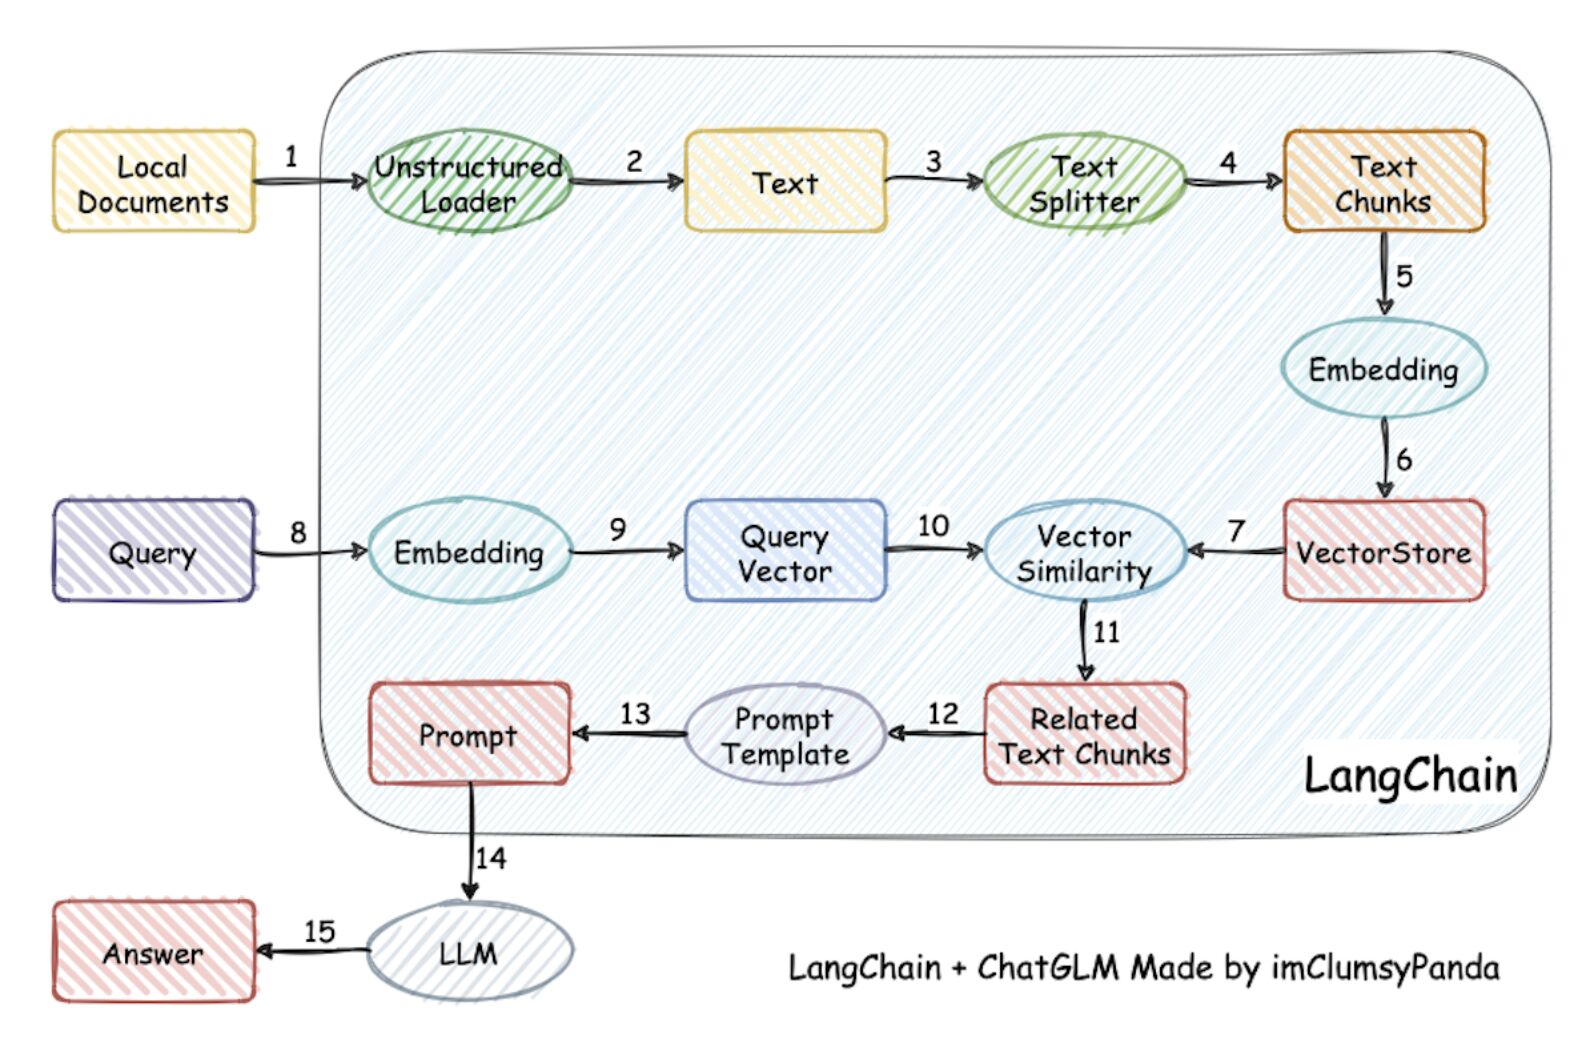
\includegraphics[width=145mm , height = 130mm]{images/major.jpeg}
    \caption{Architecture of RAG Pipleline}
    \label{fig:figure2_2}
\end{figure}
\section{Langchain}
\par  LangChain is an open-source framework designed to simplify the creation of applications using large language models (LLMs). It provides a standard interface for chains, integrates with other tools, and offers end-to-end chains for common applications. Developers can build applications based on combined LLMs (such as GPT-4) with external computation and data sources. LangChain is versatile and can be used for chatbots, code analysis, answering questions, data augmentation, text classification, summarization, and machine translation. Its key concepts include components (modular building blocks), chains (combining components), and agents (enabling LLMs to interact with their environment). LangChain has gained popularity due to its user-friendly approach and active community of contributors and users.

\subsection{Document Loaders}
\hspace{1cm} LangChain offers a versatile array of document loaders tailored to diverse data sources. From the Text Loader, adept at processing local .txt files, to the Web Page Loader, facilitating extraction from online sources, LangChain ensures seamless integration of textual data. The YouTube Transcript Loader enhances multimedia analysis by extracting transcripts from videos, while the PDF Loader enables standardized document processing. Moreover, LangChain's integration with third-party tools extends data accessibility, empowering users with a comprehensive data analysis toolkit.

\section{Embeddings Technique}
\hspace{1cm} Embeddings play a pivotal role in capturing the semantic meaning and context of textual data within LangChain. Leveraging advanced techniques such as Sentence Transformers, LangChain transforms raw text into compact yet information-rich embeddings. These embeddings serve as dense representations of the underlying document content, facilitating efficient storage, retrieval, and analysis. By utilizing Sentence Transformers, LangChain enhances the quality and effectiveness of embeddings by encoding semantic information and capturing nuanced textual relationships. This integration empowers LangChain to generate embeddings that effectively capture the semantic nuances of textual data, enabling more accurate and contextually relevant analysis and retrieval.
\section{Chunking}
\par

The RecursiveCharacterTextSplitter in LangChain efficiently breaks down documents into manageable segments for processing. Using a recursive approach, it ensures minimal information loss while handling documents of varying lengths effectively. This robust segmentation technique enhances LangChain's ability to process large volumes of text data seamlessly, enabling efficient analysis and retrieval.


\begin{figure}[ht]
    \centering
    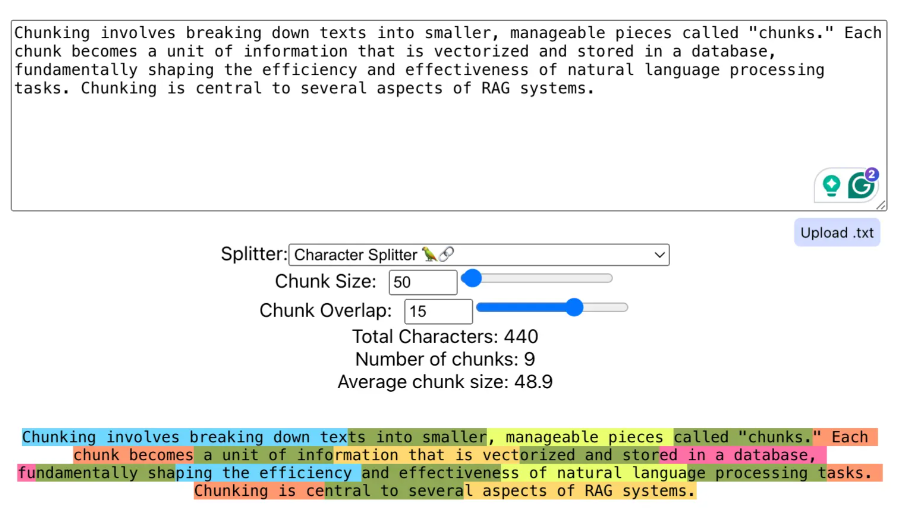
\includegraphics[width=145mm , height = 130mm]{images/chunking.png}
    \caption{Example for chunking}
    \label{fig:figure2_2}
\end{figure}

\section{Vector Store}
\par The  Chroma vector store, serves as a crucial component for efficient storage and retrieval of embeddings. The Chroma vector store specializes in storing embeddings derived from textual data, enabling quick access and retrieval during processing. It employs a robust indexing mechanism to organize embeddings, facilitating efficient search operations and retrieval of relevant information. Additionally, the Chroma vector store supports various operations such as insertion, deletion, and updating of embeddings, ensuring the integrity and scalability of the stored data. Overall, the vector store, particularly the Chroma vector store, plays a vital role in optimizing the performance and functionality of Intelligent Search Assist by providing a reliable and efficient storage solution for embeddings.


\begin{figure}[ht]
    \centering
    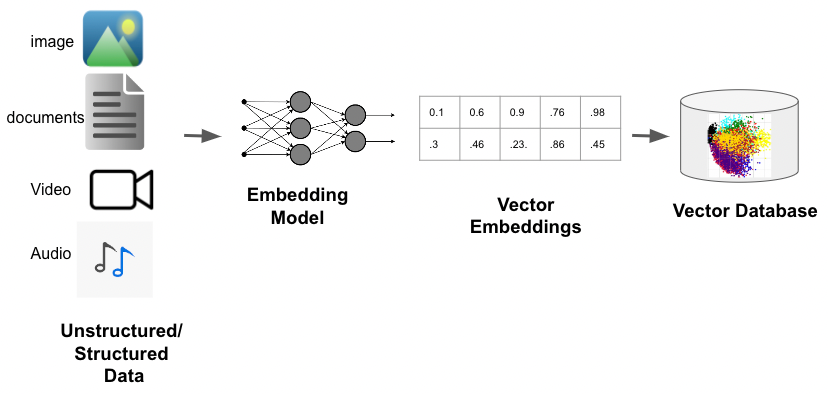
\includegraphics[width=145mm , height = 130mm]{images/vector.png}
    \caption{Vector Store}
    \label{fig:figure2_2}
\end{figure}

\section{Retrivers and chains}
\par Retrieval in LangChain is instrumental in elevating the quality of responses by efficiently fetching pertinent information based on user queries. Primarily employing semantic search, LangChain calculates numerical vectors for documents and stores them in a vector database optimized for streamlined querying. This methodology enables LangChain to retrieve documents closely aligned with the query vector, ensuring the delivery of contextually relevant results. Moreover, LangChain leverages Retrieval-Augmented Generation (RAG) techniques, amalgamating retrieval and generation processes to generate responses tailored to the context of the query.

Within LangChain, the conversation retrieval chain enhances user interaction by dynamically retrieving relevant context and documents from ongoing conversations. Initiated by a retriever component, this chain fetches pertinent documents or context based on user inputs. Subsequently, these retrieved documents, encompassing prior chat messages and context, are forwarded to a language model for response generation. This collaborative process ensures that responses are not only informed by the user's query but also enriched by contextual cues from ongoing conversations, fostering more meaningful and context-aware interactions.


\section{Prompt Template}
\par Prompt engineering is a pivotal aspect of working with language models, guiding their behavior to produce desired outputs. In LangChain, prompt templates serve as structured guides for formulating queries. These templates include instructions to the model, few-shot examples, and tailored questions, ensuring clarity and context in interactions. String prompt templates offer concise instructions, while chat prompt templates enable dynamic conversations with multiple turns and context management.

Crafting effective prompts demands a deep understanding of the task and user expectations. Well-designed prompts significantly impact the quality of model responses, requiring experimentation and iteration for fine-tuning.

\newpage
\chapter{Implementation}
\section{Data Preprocessing}
\par The initial phase of the Intelligent Search Assistant project involves processing a multitude of documents in various formats, including PDFs, Word documents, and plain text files. This diverse range of sources ensures comprehensive data intake for the system. Leveraging the robust capabilities of the LangChain framework, the system meticulously parses the text from these documents, breaking them down into manageable segments. This segmentation not only enhances processing efficiency but also facilitates a more granular understanding of the content, laying the foundation for subsequent steps in the information retrieval process.

\section{Embedding Generation}
\par Once the text segments are parsed, the system proceeds to transform them into embeddings, which serve as numerical representations of the semantic meaning of the text. This transformation is facilitated by the sophisticated Sentence Transformer technique, which excels in capturing contextual information and semantic relationships within the text segments. By generating embeddings rich in information and context, the system lays the groundwork for efficient storage and retrieval of relevant information, setting the stage for seamless user interactions.

\section{Vector Storage}
\par Efficient storage of embeddings is paramount for ensuring quick access to relevant information during user interactions. To this end, the Intelligent Search Assistant leverages LangChain's Chroma vector storage mechanism. This mechanism not only optimizes memory usage but also enhances retrieval speed, thanks to its structured organization of embeddings. By efficiently storing embeddings in a manner conducive to rapid retrieval, the system ensures responsiveness and effectiveness in addressing user queries and prompts, thereby enhancing the overall user experience.

\section{User Query Preocessing}
\par As users submit queries or prompts, the system springs into action, leveraging the Conversation Retrieval Chain to retrieve relevant documents or context. This chain seamlessly integrates retrieval techniques tailored to user input, drawing upon the stored embeddings in the Chroma vector database. By ensuring that the retrieved documents or context are contextually relevant to the user's query, the system enhances the accuracy and usefulness of the responses provided, laying the groundwork for personalized and effective interaction.
\begin{figure}[ht]
    \centering
    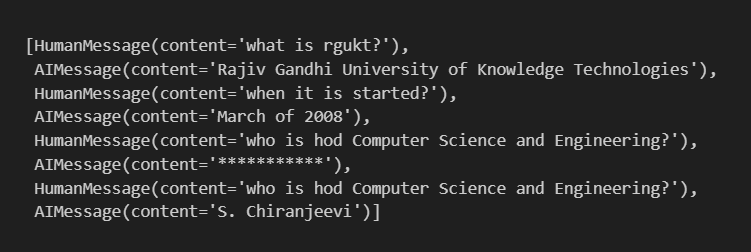
\includegraphics[width=125mm , height = 90mm]{images/rgukt-01.png}
    \caption{Q and A On Rgukt Website}
    \label{fig:figure2_2}
\end{figure}

% \begin{figure}[ht]
%     \centering
%     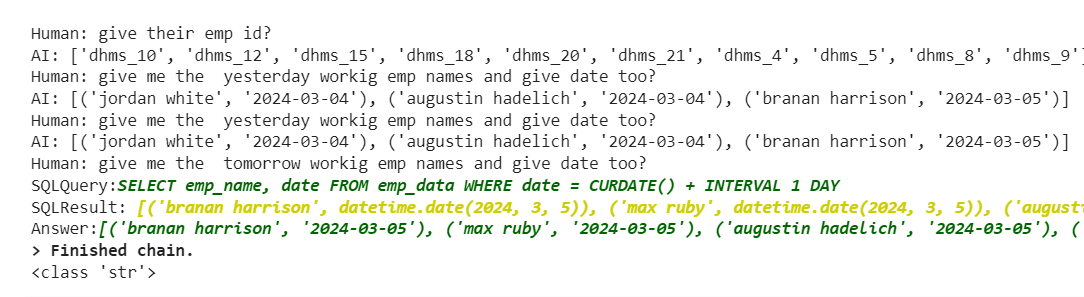
\includegraphics[width=215mm , height = 70mm]{db1.png}
%     \caption{Natural Question on the SQL Database}
%     \label{fig:figure2_2}
% \end{figure}






\newpage
\section{Google Drive Integration}
\par Google Drive integration in the Intelligent Search Assistant facilitates effortless access to files stored in users' Google Drive accounts, enhancing the efficiency of information retrieval processes. The integration begins with OAuth2 authentication to establish a secure connection with Google Drive, ensuring users' data privacy and security. Upon authentication, the system interacts with the Google Drive API to retrieve a list of files and folders, enabling users to specify the target folder for downloading files. Utilizing retrieved file metadata, the system initiates the download process from the specified folder, handling various file formats seamlessly, including documents, spreadsheets, images, and presentations.

Furthermore, the system intelligently determines the appropriate file format and extension based on the MIME type provided by Google Drive, supporting a wide range of formats such as CSV, Excel, and DOCX. To enhance reliability, a retry mechanism is incorporated for file downloads, automatically retrying the download process in case of network issues or timeouts. Additionally, robust error handling mechanisms are implemented to gracefully manage exceptions and communicate errors to users, ensuring a smooth user experience. By seamlessly integrating with Google Drive, the Intelligent Search Assistant empowers users to leverage their existing file repositories for enhanced information retrieval and analysis, thereby facilitating a streamlined workflow and improving productivity.
\hspace{10pt}

\begin{figure}[ht]
    \centering
    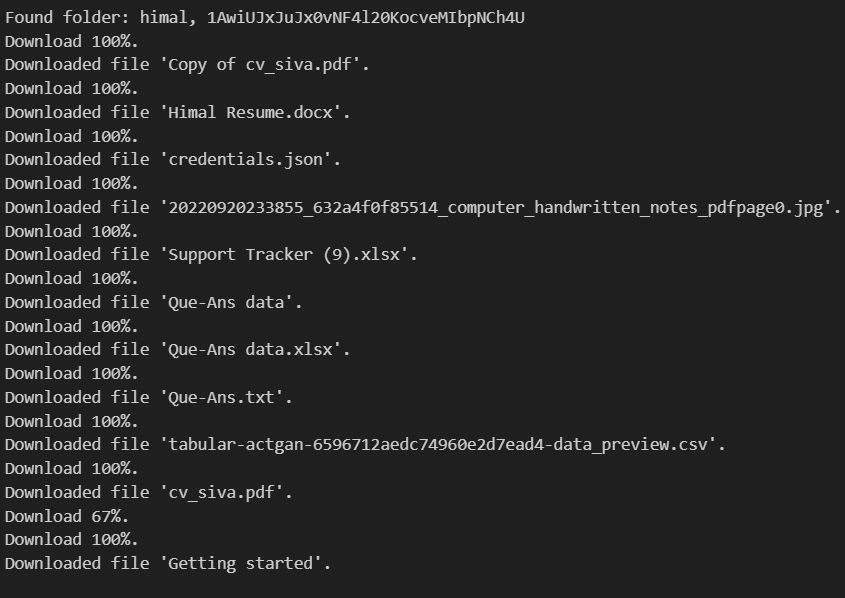
\includegraphics[width=145mm , height = 110mm]{images/google-drive.png}
    \caption{Integrating Google-drive data With Intelligent Search Assistant}
    \label{fig:figure2_2}
\end{figure}

\newpage
\chapter{Result}
\section{Result}
\par The Intelligent Search Assistant successfully integrates retrieval-augmented generation (RAG) techniques with large language models (LLMs) to deliver personalized and contextually relevant responses to user queries. Through the streamlined process of data preprocessing, embedding generation, and vector storage, the system efficiently organizes and retrieves information from diverse sources, including documents, websites, and multimedia content. Leveraging the LangChain framework and the Sentence Transformer technique, the system transforms textual data into compact embeddings, facilitating quick retrieval and response generation.

Moreover, the integration with Google Drive enables seamless access to users' files, enhancing the breadth and depth of information available for retrieval. By intelligently parsing file metadata and employing robust download mechanisms, the system ensures smooth and reliable access to various file formats, including documents, spreadsheets, images, and presentations. The result is an intelligent search assistant that empowers users to access and analyze information from their Google Drive repositories with ease, ultimately improving productivity and facilitating informed decision-making.

\section{Sample Output Screenshots}

\begin{figure}[ht]
    \centering
    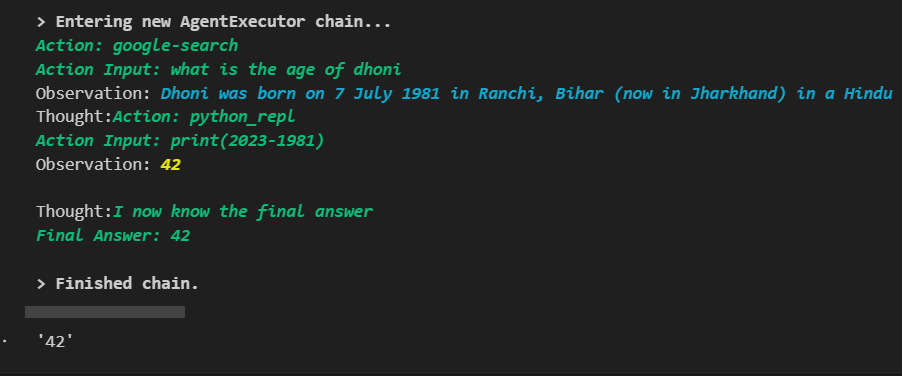
\includegraphics[width=145mm , height = 110mm]{Dhoni.png}
    \caption{Making LLM models Up to date with Lagnchain agent}
    \label{fig:figure2_2}
\end{figure}


\section{Requirements}
\subsection{Software Requirements}
\begin{itemize}
\item{LangChain}
\item{Embeddings Techniques}
\item{Retrieval-Augmented Generation (RAG) techniques}
\item{Large Language Models (LLMs)}
\item{Vector Databases}
\item{Python}
\end{itemize}

\subsection{Hardware Requirements}

\begin{itemize}
\item{Modern Operating System}
\item{4 GB RAM}
\item{10 GB Free Disk Space}
\item{X86 64-bit CPU(Intel/AMD Architecture)}
\end{itemize}




\newpage
\chapter{Future Scope}
\textbf{    Integrating More Data Storage Platforms:} By incorporating additional data storage platforms like Slack, OneDrive, and Dropbox, you can enhance the accessibility and versatility of your Intelligent Search Assistant, allowing users to retrieve information from a wider range of sources.

\textbf{Implementing Efficient Chunking Techniques:} Introducing advanced chunking techniques such as semantic chunking can improve the organization and retrieval of information within the system, leading to more accurate and relevant search results for users.


\textbf{Creation of Web Application Using ChainLit Python Framework:} Developing a web application using the ChainLit Python framework can make your Intelligent Search Assistant more accessible to users across different platforms and devices, expanding its reach and usability.

\textbf{Local Project with LLM Model Download:} Enable users to run the Intelligent Search Assistant locally by downloading the LLM model, providing greater control and flexibility, especially in environments with limited internet access or privacy concerns.

\textbf{Converting Application into No-Code Platform:} TTransform the application into a no-code platform, allowing users to easily build customized assistants using drag-and-drop functionality, democratizing access to AI-powered information retrieval tools for users with varying technical expertise.
\newpage
\chapter{Conclusion}
\hspace{20pt}In conclusion, the Intelligent Search Assistant represents a significant advancement in information retrieval systems, leveraging cutting-edge technologies such as LangChain, large language models (LLMs), and retrieval-augmented generation (RAG) techniques. Through seamless integration with various data sources including Google Drive and robust document preprocessing methods, the system offers users a personalized and efficient means of accessing relevant information. The future scope of the project, including integration with additional storage platforms, implementation of advanced chunking techniques, and conversion into a no-code platform, promises further enhancements in usability and accessibility. Overall, the project showcases the potential of AI-driven solutions to revolutionize user interaction and streamline information retrieval processes.

\newpage
\chapter{Refernece}
\begin{itemize}
\item{https://python.langchain.com/docs/}
\item{https://cloud.google.com/docs}
\item{https://www.analyticsvidhya.com/blog/2023/09/retrieval-augmented-generation-rag-in-ai/}
\item{https://docs.trychroma.com/usage-guide)}
\item{https://huggingface.co/docs}
\item{https://docs.llamaindex.ai/en/stable/}
\end{itemize}


\end{document}